%preamble
\documentclass[12pt,a4paper]{article}

%inputs for firstpage
\def \CourseName {گزارش فاز دوم}
\def \Instructor {دکتر مسلم حبیبی}
\def \Semester {نیم‌سال دوم\\سال تحصیلی 99-00}


%packages
\usepackage[]{algorithm2e}
\usepackage{cite}
\usepackage{calc}
\usepackage{fancyhdr}
\usepackage{lipsum}
\usepackage{color}
\usepackage{ragged2e}
\usepackage[inline]{enumitem}
\usepackage[dvipsnames]{xcolor}
\usepackage{graphicx}
\usepackage{wrapfig}
\usepackage{float}
\usepackage[skip=12pt,indent=2em]{parskip}
\usepackage{setspace}
\usepackage{textcomp}
\usepackage{etoolbox}
\usepackage{xpatch}
\usepackage{tabu}
\usepackage{hyperref}


%for persian fonts
\usepackage{xepersian}
\defpersianfont\bnazanin{BNazanin}
\settextfont{BNazanin}

\title{
	\center
	
\includegraphics[width=5cm, height=5cm]{images/shariflogo.jpg} \\
	دانشکده مهندسی صنایع \\
	دانشگاه صنعتی شریف \\
	\CourseName
}
\author{
	\\
	\\
	\textbf{استاد درس:}
	\\
	\Instructor \\[35pt]
	\\
	\textbf{نام اعضای گروه:}
	\\مهدی محسنی 
	\\محراب کشاورز گیلده 
	\\احسان چشمی
	\\[45pt]
}
\date{{\small\Semester}}


%body
\begin{document}

\maketitle
\pagebreak
\tableofcontents
\pagebreak
\listoffigures
\pagebreak
\normalsize	

\section{نمودار موردکاربرد} \label{section.useCase}
	\begin{figure}[h!]
		\begin{center}
			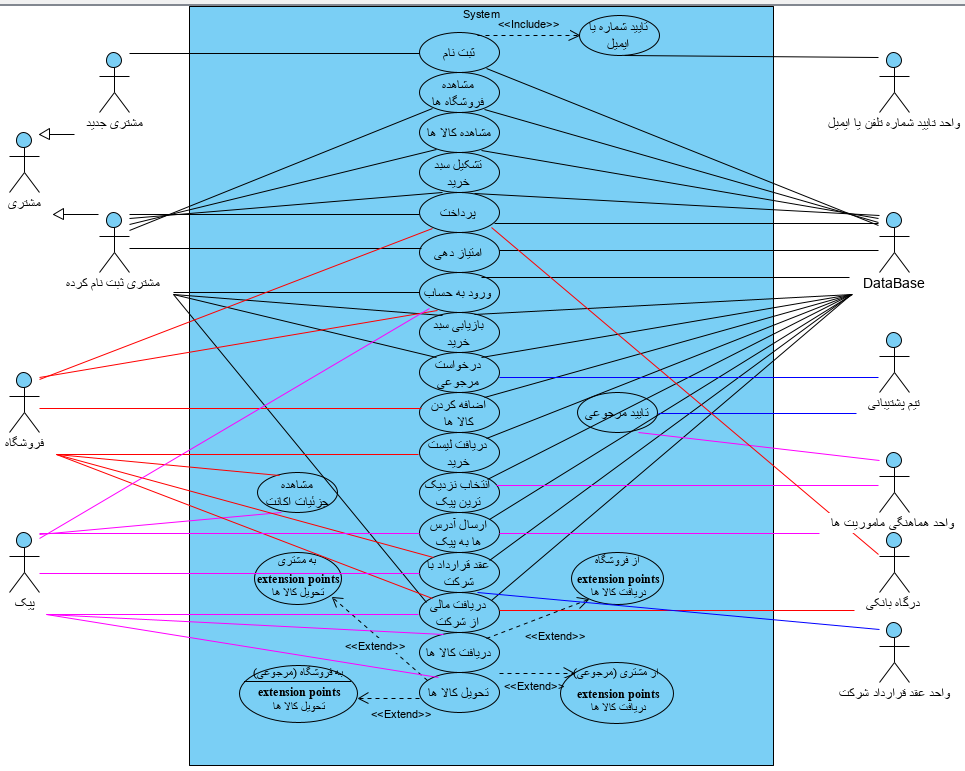
\includegraphics[width=12cm]{images/Use Case.png}
			
		\end{center}
		\caption{نمودار مورد کاربرد}
	\end{figure}
 

\textbf{توضیحات :} 
	\begin{enumerate}
		\item 
		آکتورهای مشتری جدید و مشتری ثبت نام شده را با یک رابطه ارث بری به آکتور والد مشتری متصل می کنیم.
		\item
		فرض بر این بوده که مشتری تنها بعد ثبت نام میتواند لیست فروشگاه ها و کالاها را ببیند.
		\item
		منظور از یوزکیس بازیابی سبد خرید، بعد از پرداخت ناموفق است.
		\item
		فرض بر این بوده تمام دیتاها از جمله موجودی کالاها، جزییات حساب ها، تاریخچه پرداخت ها و غیره در دیتابیس شرکت ذخیره می شود.
		\item
		منظور از یوزکیس دریافت مالی از شرکت دریافت مبلغ فروش توسط فروشگاه،درآمد پیک از تحویل کالا و مبلغ بازگشتی به مشتری در صورت مرجوع کردن کالا می باشد.
		\item
		آکتور واحد هماهنگی ماموریت ها وظیفه دریافت اطلاعات پیک ها از دیتابیس شرکت، پیدا کردن نزدیکترین پیکی که ماموریت را بپذیرد، و سپردن ماموریت دریافت و تحویل کالا به پیک را دارد.
	\end{enumerate}
\pagebreak
\section{نمودارهای فعالیت} \label{section.activity}
	\subsection{فرایند ثبت نام} \label{section.activity.register}
		\begin{figure}[h!]
			\begin{center}
				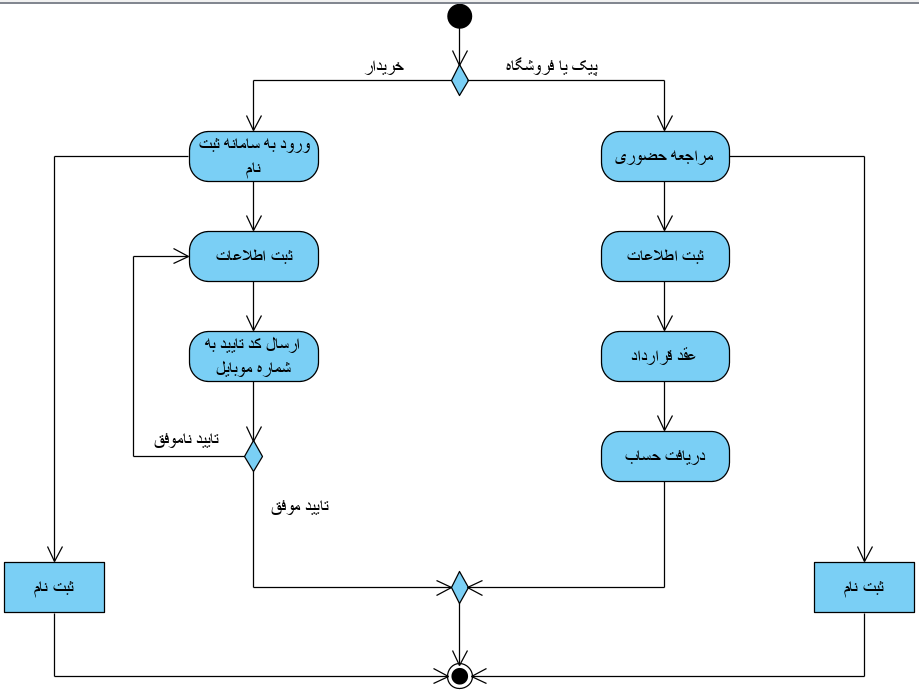
\includegraphics[width=14cm]{images/Register Activity Diagram.png}
			\end{center}
			\caption{نمودار فعالیت ثبت نام}
		\end{figure}
	
	\textbf{توضیحات :} 
	
	
	خریدار برای ثبت نام وارد سامانه می شود، اطلاعات خود را وارد میکند و کد تایید به شماره یا ایمیل او ارسال می شود. در صورت عدم تایید شماره یا ایمیل دوباره به مرحله ثبت اطلاعات بازمی گردد و در صورت تایید ثبت نام تایید می گردد.	پیک یا صاحب فروشگاه برای ثبت نام به صورت حضوری مراجعه می کنند، اطلاعات خود را به متصدی ثبت نام می دهند و قرار داد امضا می کنند سپس حساب کاربری خود در سامانه را دریافت می کنند.
\pagebreak	
	\subsection{فرایند خرید} \label{section.activity.buy}
	\textbf{توضیحات :} 
	
	
	کاربر وارد سامانه می شود از اینکه ممکن است در ورود به سامانه مشکل برایش پیش بیاید (مثلا رمز عبور را اشتباه بزند)، صرف نظر شده است. لیستی از فروشگاه های نزدیک به او نشان داده می شود. فروشگاه مدنظرش را انتخاب می کند. در اینجا فرض شده که لیستی از تمام فروشگاه ها به او نشان داده می شود و فقط ترتیب نمایش آن ها این گونه است که فروشگاه های نزدیک به او در اولویت هستند. بعد از اینکه فروشگاه را انتخاب کرد وارد صفحه ی آن فروشگاه می شود و لیست کالاهای آن را می بیند. سپس اگر کالا یا کالاهای مدنظرش را یافت آن ها در سبد خریدش وارد می کند. فرض شده که کاربر در سبد خرید فقط می تواند از یک فروشگاه محصول داشته باشد. مثلا اگر او بخواهد از یک فروشگاه کفش بخرد و از فروشگاه دیگری لباس بخرد باید یک بار کفش را بخرد و سفارش اش را تکمیل کند و بعد از آن دوباره لباس در سبد خریدش اضافه کند. بعد از وارد کردن تعداد و نوع محصولات فرد سبد خریدش را چک می کند. اگر حاضر به خرید آن سبد نباشد یا کلا منصرف می شود که در این صورت از سامانه خارج می شود و سبد خریدش حذف می شود یا اینکه می خواهد در محصولات انتخابی تغییری دهد. در این حالت نیز سبد خریدش حذف می شود. اما اگر حاضر به خرید سبد شد آن را تایید می کند سپس سبد توسط سیستم چک می شود. اگر مشکلی وجود داشت پیام خطا داده می شود و کاربر باید سبد را دوباره بچیند اما اگر مشکلی نبود کاربر به صفحه ی درگاه بانکی انتقال پیدا می کند و بعد از وارد کردن اطلاعات و واریز وجه باید منتظر تایید درگاه بماند. اگر پرداخت ناموفق باشد لیست خرید کاربر ذخیره می شود و اگر پرداخت موفق باشد لیست خرید به سامانه ارسال می شود. بعد از آن دو فعالیت همزمان انجام می شود به این نحو که سامانه به دنبال نزدیک ترین پیک می گردد و در همان زمان لیست سفارش برای فروشگاه ارسال می شود. بعد از آن فروشگاه سفارش را آماده می کند. بعد از اینکه نزدیک ترین پیک پیدا شد درخواستی به او ارسال می شود اگر پیک این درخواست را قبول کند باید برود و سفارش را از فروشگاه تحویل بگیرد و بعد به مشتری بدهد اما اگر قبول نکند سامانه به دنبال پیک دیگری خواهد گشت.
	
	\pagebreak		
	\subsection{فرایند مرجوعی} \label{section.activity.return}
		\begin{figure}[h!]
			\begin{center}
				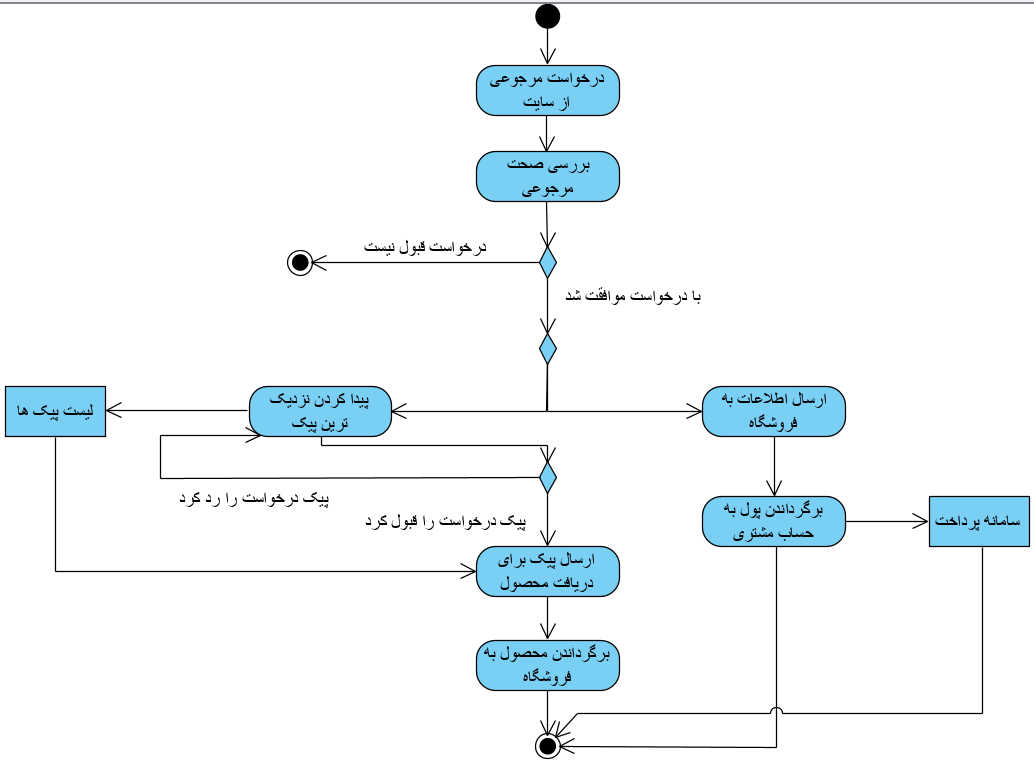
\includegraphics[width=14cm]{images/Return Activity Diagram.png}
			\end{center}
			\caption{نمودار فعالیت مرجوعی}
		\end{figure}
		
	\textbf{توضیحات :} 
	
	
	پس از بررسی صحت درخواست مرجوعی مشتری در صورتی که درخواست غیر منطقی باشد و قابل قبول با قوانین تایید شده در هنگام خرید نباشد درخواست رد می شود در غیر این صورت درخواست قبول می شود و دو اتفاق می افتد:
	\begin{enumerate}
		\item
		اطلاعات مرجوعی به فروشگاه داده می شود تا پول را پس دهد.
		\item
		نزدیک ترین پیک پیدا می شود تا محصول را از مشتری دریافت کند و به فروشگاه برگرداند.
	\end{enumerate}
	\textbf{نکته: }دو قسمت \underline{لیست پیک ها }و \underline{سامانه پرداخت} آبجکت هستند و اتصال به آن ها باید با خط چین باشد اما ویژوال پارادایم آن ها را خط گذاشته است.
	
\pagebreak

\section{نمودارهای توالی} \label{section.sequence}

	
	\subsection{فرایند ثبت نام} \label{section.sequence.register}
		\begin{figure}[h!]
			\begin{center}
				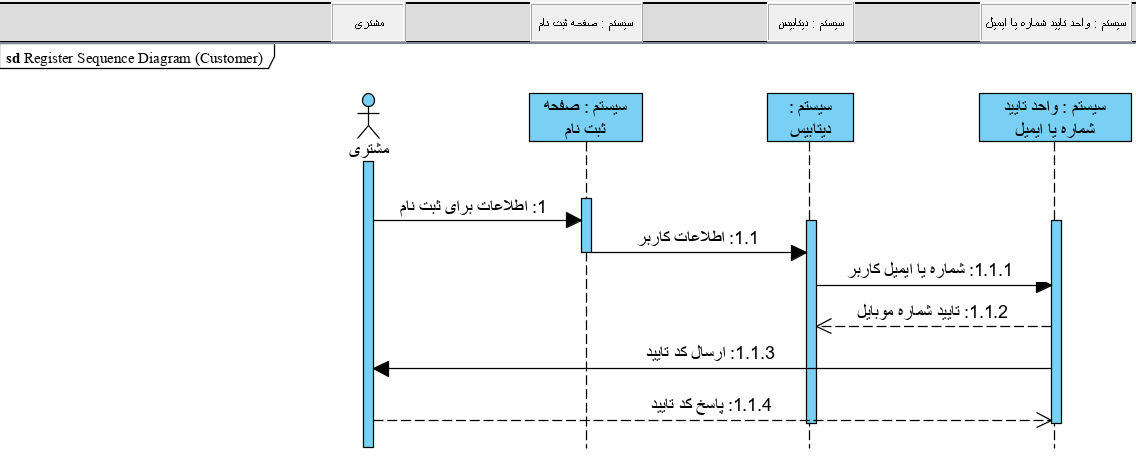
\includegraphics[width=12cm]{images/Register Sequence Diagram (Customer).png}
			\end{center}
			\caption{نمودار توالی ثبت نام - مشتری}
		\end{figure}
		
		\begin{figure}[h!]
			\begin{center}
				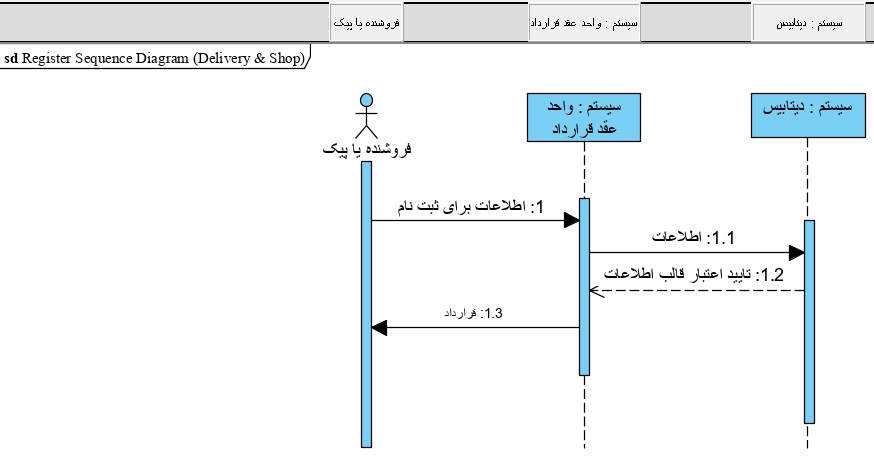
\includegraphics[width=12cm]{images/Register Sequence Diagram (Delivery & Shop).png}
			\end{center}
			\caption{نمودار توالی ثبت نام - فروشگاه و پیک}
		\end{figure}
		
		\textbf{توضیحات :} 
		
		
	خریدار برای ثبت نام وارد سامانه می شود، اطلاعات خود را وارد میکند و کد تایید به شماره یا ایمیل او ارسال می شود. در صورت عدم تایید شماره یا ایمیل دوباره به مرحله ثبت اطلاعات بازمی گردد و در صورت تایید ثبت نام تایید می گردد.	پیک یا صاحب فروشگاه برای ثبت نام به صورت حضوری مراجعه می کنند، اطلاعات خود را به متصدی ثبت نام می دهند و قرار داد امضا می کنند سپس حساب کاربری خود در سامانه را دریافت می کنند. تمامی اطلاعات در دیتابیس ثبت می شود.	
		\pagebreak
	
	\subsection{فرایند خرید} \label{section.sequence.buy}
	\textbf{توضیحات :}
	فرضیات و توضیحات نمودار فعالیت در اینجا صادق است. جز اینکه فرض شده تمام اطلاعات در دیتابیس ها ذخیره می شود و با خروج کاربر از سامانه سبد خرید حذف نمی شود.
	رابط کابری سامانه (  اپلیکیشن یا وبسایت) برای همه کاربران (مشتری، فروشنده، پیک) یک آبجکت فرض شده.
	فرض شده که سبد همواره در مرحله بررسی تایید می شود.
	
	
	\subsection{فرایند مرجوعی} \label{section.sequence.return}
		\begin{figure}[h!]
			\begin{center}
				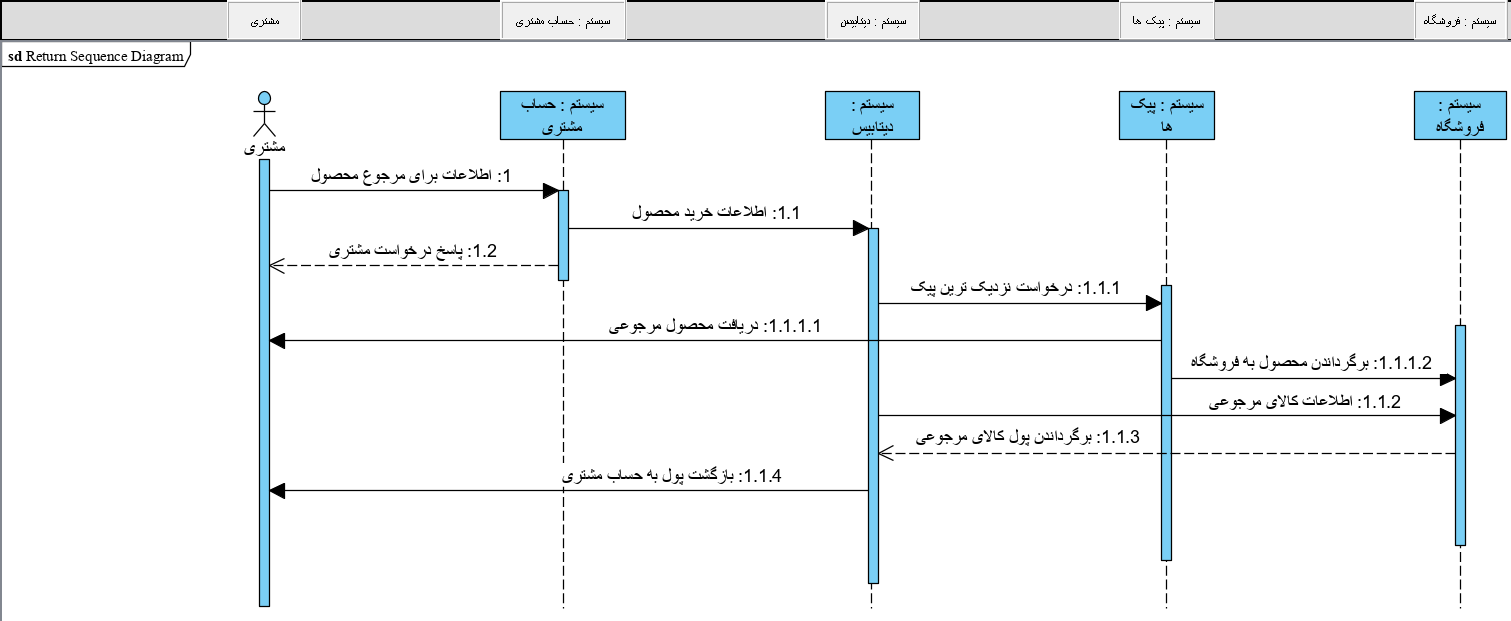
\includegraphics[width=14cm]{images/Return Sequence Diagram.png}
			\end{center}
			\caption{نمودار توالی مرجوعی}
		\end{figure}
		
		\pagebreak
	

\pagebreak

\section{گزارش نحوه انجام پروژه} \label{section.report}
	دو روز بعد از اتمام فاز اول جلسه ی پس از مرگ \footnote{\lr{post mortem}} در محیط اسکایپ \footnote{\lr{Skype}}انجام شد و پس از آن جلسه و باتوجه به نتایج بدست آمده از آن، هر سه عضو گروه با هم کارهای مربوط به فاز دوم پروزه را تفکیک و بین یکدیگر تقسیم کردیم و بنابر این شد که \underline{مهدی محسنی} این تقسیم وظایف را در گیت هاب\footnote{\lr{https://github.com/}} وارد کند. برنامه ریزی انجام شده از این قرار بود که در اسپرینت دوم اعضای گروه مطالب مورد نیاز برای انحام فاز دوم را بخوانند و فعالیتی برای اعضا در اسپرینت دوم در نظر گرفته نشد! دلیل این کار، مشغولیت زیاد درسی اعضا بود و نمی شد علاوه بر خواندن میانترم های دیگر و انجام پروژه ی درس های دیگر وقت بیشتری برای این پروژه گذاشت. باتوجه به مطالب بیان شده این پروژه برنامه ریزی شد که در عرض 3 اسپرینت به اتمام برسد:
	\begin{center}
		\begin{tabular}{|c|c|} 
			\hline
			\textbf{اسپرینت 2 } & خواندن و آموختن مطالب مورد نیاز برای انجام فاز دوم\\
			\hline
			\hline
			\textbf{اسپرینت 3 } & کشیدن نمودارهای مورد نیاز این فاز روی کاغذ و  نوشتن توضیحات آن ها \\
						 & به علاوه ی عکس نمودارها در فایل ورد مورد نظر در گیت هاب \\
			\hline
			\hline
			\textbf{اسپرینت 4} & کشیدن نمودارها به کمک نرم افزار و نوشتن گزارش فاز دوم در لاتک\\
			\hline
		\end{tabular}
	\end{center}


در اسپرینت دوم اعضای گروه توانستند که مطالب مورد نیاز را فرابگیرند اما در اسپرینت سوم تمامی نمودارها تکمیل نشد و نمودارهای فعالیت و توالی خرید در اسپرینت بعدی انجام شدند. وظایف سپرده شده به اعضای گروه در اسپرینت چهارم\footnote{زمان این اسپرینت تا روز تحویل پروژه است. با توجه به تمدید پروژه، ما به جای اضافه کردن یک اسپرینت دیگر، این اسپرینت را طولانی تر کردیم.} که مربوط به این فاز می شد به طور کامل و به موقع انجام شد. 


\textbf{نکته :} متاسفانه در این فاز نیز مانند فاز قبل اعضای گروه به \lr{commit} و \lr{push} کردن مطالب اکتفا کردند و فراموش کردند که مشکلی\footnote{\lr{issue}} که به آن ها اختصاص داده شده بود را بعد از انجام دادن ببندند به همین دلیل تمامی مشکلات در گیت هاب توسط \underline{مهدی محسنی} و در یک زمان بسته شد اما این موضوع به این معنی نیست که همه ی آن ها در یک روز انجام شده باشد. این مطلب حتی در جلسه ی پس از مرگ نیز ذکر شد اما باز هم اعضای گروه فراموش کردند.

\pagebreak
	\subsection{\lr{Task board and Burndown Chart}} \label{section.report.taskBoard}
			\begin{figure}[h!]
			\begin{center}
				\includegraphics[width=9cm]{images/screenshot_1.png}	
			\end{center}
			\caption{ابتدای اسپرینت-بخش اول}
		\end{figure}
		
		\begin{figure}[h!]
			\begin{center}
				\includegraphics[width=9cm]{images/screenshot_2.png}
			\end{center}
			\caption{ابتدای اسپرینت-بخش دوم}
		\end{figure}
			\begin{figure}[h!]
			\begin{center}
				\includegraphics[width=9cm]{images/screenshot_3.png}	
			\end{center}
			\caption{ابتدای اسپرینت-بخش سوم}
		\end{figure}
		
		\begin{figure}[h!]
			\begin{center}
				\includegraphics[width=9cm]{images/screenshot_4.png}
			\end{center}
			\caption{انتهای اسپرینت-بخش اول}
		\end{figure}
			\begin{figure}[h!]
			\begin{center}
				\includegraphics[width=9cm]{images/screenshot_5.png}	
			\end{center}
			\caption{انتهای اسپرینت-بخش دوم}
		\end{figure}
		
		\begin{figure}[h!]
			\begin{center}
				\includegraphics[width=9cm]{images/screenshot_6.png}
			\end{center}
			\caption{انتهای اسپرینت-بخش سوم}
		\end{figure}
	
	\pagebreak
	
	
	\begin{figure}[h!]
		\begin{center}
			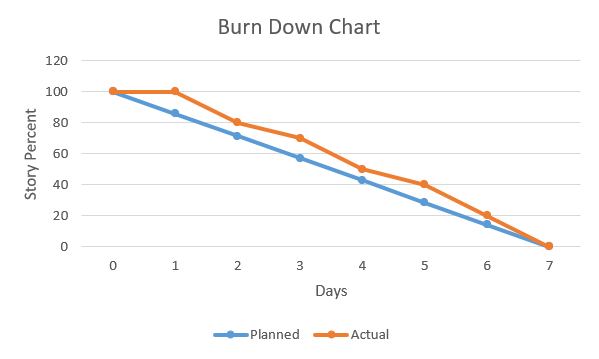
\includegraphics[width=14cm]{images/Burn Down Chart.png}
			
		\end{center}
		\caption{\lr{Burn Down Chart}}
	\end{figure}
	
	
	

\end{document}